\documentclass[11pt]{article}
\usepackage[margin=1in]{geometry}\usepackage{graphicx}\usepackage{parskip}\usepackage{hyperref}
\title{Spatial Degradation of Hepatocyte Zonation in Human MASLD\\
\large An analysis report: building, validating and transferring a zonation ruler}
\author{}\date{2026-06-21}
\begin{document}\maketitle

\section{Background and question}
The liver lobule is spatially organized along a porto-central axis: pericentral hepatocytes (near
the central vein) and periportal hepatocytes (near the portal triad) run complementary metabolic
programs, and most hepatocyte genes are \emph{zonated}. \textbf{Paper~2} (Yakubovsky \& Itzkovitz,
\emph{Nature} 2026) built a spatially resolved atlas of the \emph{healthy} human liver and a
quantitative zonation reference. \textbf{Paper~1} (Gribben, Vallier et al., \emph{Nature} 2024,
GSE202379) profiled $\sim$69k hepatocytes by single-nucleus RNA-seq across 47 donors spanning
MASLD stages (Healthy $\to$ NAFLD $\to$ NASH $\to$ Cirrhosis $\to$ End-stage), but is
\emph{spatially blind}. Paper~1 reports qualitatively that ``hepatocytes lose their zonation''.

This project makes that quantitative. We use Paper~2's healthy zonation as a \emph{ruler} to assign
each Paper~1 hepatocyte a pseudo-zonation coordinate, then test, at the level of the \textbf{donor}
(never the cell, to avoid pseudoreplication):
\begin{itemize}
\item \textbf{H1}: does zonation collapse with disease stage?
\item \textbf{H2}: which gene programs lose their zonal restriction (slope), and fastest?
\item \textbf{H3}: are de-zonated cells also more plastic (hepatocyte$\leftrightarrow$cholangiocyte)?
\end{itemize}

\section{Method, and the one rule that governs it}
A ruler is any rule that maps a cell's transcriptome to a porto-central coordinate. We compared
many: Paper~2's exact 20+20 \emph{landmark} genes; curated anchor sets; data-driven top-$N$ and
``full'' sets ranked from Paper~2's zonation table; a \emph{learned} dense PCA axis; sparse
\emph{lasso}/\emph{elastic-net} axes; and a supervised whole-transcriptome classifier. Each yields
coord $=\mathrm{mean\_z}(\mathrm{PC})-\mathrm{mean\_z}(\mathrm{PP})$ or a learned projection.

\textbf{The governing rule: ruler quality is judged ONLY on the healthy atlas} --- an 8-marker
sign gate (pericentral CYP2E1/CYP1A2/GLUL/PCK2 must correlate $+$; periportal ASS1/ALDOB/PCK1/HAL
$-$), the healthy PC--PP anti-correlation (a real axis has the two arms mutually exclusive), and
split-half reproducibility. The best healthy ruler is \emph{frozen} and only \emph{then} applied to
the disease cohort. Disease H1/H2/H3 are the \emph{test}; they are never used to choose a ruler.
Choosing by disease strength would be circular (leakage).

\subsection{Statistical tests --- what each checks, and how}
Every test follows the donor rule: collapse each donor's cells to one number, then test on the
$\approx$47 donor values (resampling/permuting donors, never cells). Tests are rank-based by default
(ordinal stages, skewed scores, small $n$); effect sizes are reported beside every $p$; BH-FDR
controls multiple testing.

\begin{tabular}{l l l}
\hline
test & what it checks & how \\
\hline
Spearman $\rho$ & monotone trend of a metric vs stage & rank correlation; donor-level \\
Jonckheere--Terpstra & ordered-groups trend (dedicated) & $J=\sum_{a<b}U_{ab}$, permutation $p$ \\
Donor bootstrap CI & how big / how sure the trend is & resample donors $B{=}2000$, 2.5/97.5 pct \\
Label-shuffle perm. & is the pipeline finding noise? & shuffle stage labels, recompute \\
Held-out gene split & H2 without circularity & build coord on half genes, test other half, $K{=}20$ \\
Mann--Whitney $U$ (H2b) & does a program weaken $>$ background? & $U$ of program vs rest, rank-biserial, BH-$q$ \\
Per-gene FDR (H2c) & which individual genes lose slope & Spearman per gene, BH over $\sim$30k \\
Within-donor corr (H3) & dez$\leftrightarrow$plast, stage-free & $\rho_d$ per donor; sign test \& Wilcoxon vs 0 \\
Mann--Whitney AUC (H3) & dez vs zonated plasticity & within-donor AUC, aggregate \\
OLS + C(stage)+C(donor) & partial dez effect (descriptive) & coefficient on dez (cell-level SE) \\
\hline
\end{tabular}

\section{Results and analysis}

\subsection{Not every ruler is a ruler: a dilution curve}
The 8-marker gate passes for almost everything (the markers are strong), but it is not sufficient.
The decisive control is the \emph{healthy PC--PP anti-correlation}. Small, high-SNR sets are
genuinely bipolar (\texttt{paper2\_landmark}: $-0.45$; \texttt{expanded\_curated}: $-0.48$), but as the gene set grows the axis
degrades and finally inverts: \texttt{paper2\_top250} $\approx +0.04$, \texttt{paper2\_full} $\approx +0.55$. Averaging
$\sim$2000 weakly-zonated genes lets a shared technical/expression factor dominate, so the
``full'' coordinate is \emph{not} a zonation axis at all. This is why a transcriptome-wide
\emph{unweighted} mean fails while a \emph{weighted} or selected ruler succeeds.

\subsection{Ruler ranking and selection (healthy metrics ONLY)}
Every ruler is scored on \textbf{healthy} quality alone --- a quality score of
(split-half reproducibility) $+\,\max(0,-$healthy PC--PP anticorrelation$)$ --- and the table below
is \textbf{ordered by it}. Disease-collapse strength is deliberately \emph{excluded} from selection:
using the test cohort to choose the instrument would be leakage. The frozen primary is the
top-ranked \emph{published-signature} set; learned rulers are shown for comparison but do not compete
in the auto-selection. We keep the whole spectrum (curated, data-ranked, learned PCA, regularized,
supervised) because agreement of \emph{independent construction mechanisms} is the robustness
evidence --- not because any one is cherry-picked.

\begin{tabular}{l r r r r r l}
\hline
ruler & PC & PP & healthy anticorr & split-half & H1 spread $\rho$ & role \\
\hline
unsupervised\_combined & 4769 & 3719 & -0.50 & 0.72 & -0.51 & primary\_candidate \\
unsupervised\_p2 & 5177 & 3302 & -0.47 & 0.69 & -0.50 & primary\_candidate \\
expanded\_curated & 26 & 23 & -0.48 & 0.67 & -0.43 & primary\_candidate \\
selected\_frozen & 26 & 23 & -0.48 & 0.67 & -0.43 & primary\_candidate \\
unsupervised\_top100 & 100 & 100 & -0.29 & 0.82 & -0.61 & primary\_candidate \\
unsupervised\_top50 & 50 & 50 & -0.31 & 0.79 & -0.62 & primary\_candidate \\
unsupervised & 4585 & 3903 & -0.31 & 0.78 & -0.56 & primary\_candidate \\
paper2\_landmark & 20 & 20 & -0.45 & 0.63 & -0.38 & primary\_candidate \\
unsupervised\_top250 & 250 & 250 & -0.23 & 0.85 & -0.57 & primary\_candidate \\
paper2\_top50 & 50 & 50 & -0.40 & 0.57 & -0.32 & primary\_candidate \\
paper2\_top100 & 100 & 100 & -0.27 & 0.56 & -0.28 & primary\_candidate \\
unsupervised\_full & 4585 & 3903 & 0.65 & 0.83 & -0.42 & exploratory \\
core\_curated & 13 & 8 & -0.28 & 0.54 & -0.54 & interpretability\_only \\
unsupervised\_lasso & 126 & 149 & -0.18 & 0.63 & -0.51 & robustness \\
unsupervised\_elasticnet & 325 & 281 & -0.07 & 0.69 & -0.49 & robustness \\
paper2\_top250 & 250 & 250 & 0.04 & 0.55 & -0.27 & exploratory \\
paper2\_full & 1624 & 447 & 0.56 & 0.48 & -0.04 & exploratory \\
full & 0 & 0 & 0.53 & 0.46 & 0.02 & exploratory \\
supervised & 4504 & 3935 & -0.01 & 0.45 & 0.12 & exploratory \\
\hline
\end{tabular}

\subsection{Which ruler we selected, and why it is not the strongest-on-disease one}
By healthy-ruler quality the selected primary set is \texttt{expanded\_curated}. Notably this is \emph{not} the
set with the strongest disease trend (the small curated \texttt{core\_curated} set has a steeper collapse) ---
choosing that would be cherry-picking. Selection used healthy metrics only; the disease result is
the independent confirmation.

\subsection{H1 --- zonation collapses (and it is robust)}
On every \emph{valid} ruler, per-donor coordinate spread falls and the PC--PP anti-correlation
rises toward zero across stages. The signal is concentrated and reproducible:
landmark spread $\rho=-0.380$ (perm $p=0.0085$); expanded $\rho=-0.434$; the label-free dense
PCA axis $\rho=-0.562$ (perm $p=0.0005$). The broken ``full'' ruler is null ($\rho=-0.042$),
exactly as its healthy diagnostics predicted. The agreement of the published-signature ruler and a
\emph{label-free} ruler is the key point: the collapse is a property of the data, not of any one
gene list.

\paragraph{Early disease is the noisy part (stated honestly).} The decline is \emph{not} strictly
monotonic from Healthy: at NAFLD the coordinate is often as zonated as (or slightly more than)
Healthy, and the Healthy$\to$NAFLD \emph{direction flips across rulers} (up for landmark/expanded,
down for the dense PCA axis) --- exactly the instability expected where the signal is weakest and $n$
smallest (Healthy $n=4$, NAFLD $n=7$). All rulers nonetheless \emph{agree} on the strong
NASH$\to$end-stage decline. So the defensible claim is an ordered collapse \emph{across the disease
course, driven by NASH$\to$end-stage}, with early steatosis leaving zonation largely intact ---
consistent with steatosis beginning pericentrally before inflammation and fibrosis dissolve the axis.

\subsection{Leakage control --- the unsupervised axis is clean}
A fair concern: was the learned axis trained on disease cells? No. It was learned on healthy cells
only and frozen. To remove all doubt we also trained the axis \emph{entirely on the external
Paper~2 healthy atlas} (zero Paper~1 cells in fitting) and transferred it: the collapse survived
($\rho=-0.50$, $p=3\times10^{-4}$, 8/8 markers). And the label-free PCA axis correlates $\rho=+0.57$ with the landmark-signature coordinate ($\rho=+0.39$ with its PC arm, $-0.45$ with its PP arm) --- so the axis is not a
signature-formula artefact, and the result is not a variance-maximization artefact.

\subsection{H2 --- which programs lose zonation, and fastest}
\textbf{H2a (held-out slope-loss).} Building the coordinate from one random half of the ruler genes
and testing the other half (repeated $K{=}20\times$), most held-out genes lose their donor-level
zonal slope with disease (e.g.\ 96/100 weaken for the unsupervised ruler) --- a non-circular
confirmation that the genes defining zonation flatten with disease.

\textbf{H2c (transcriptome-wide, per gene).} Taking it further: assign every cell the frozen ruler
coordinate and test \emph{all} 29969 genes' donor-level zonal slope. 67\,\% lean toward
weakening (a real directional bias --- pure noise would give 50\%), \emph{but only 8 survive
BH-FDR} at $q<0.05$. Why so few? Each gene's slope is estimated per donor from a handful of zone
bins, and with only $n{=}47$ donors the per-gene test is weak; correcting across $\sim$30k genes,
almost no single gene is individually a stand-out. So the collapse is \textbf{broad and diffuse} ---
most genes lose a \emph{little} zonation rather than a few master genes losing a lot.

\textbf{H2b (program-level --- where the power and the structure are).} Diffuse does \emph{not} mean
uniform. Grouping genes into programs and aggregating recovers the power that per-gene FDR throws
away: for each program we test, by Mann--Whitney $U$, whether its genes weaken \emph{more than the
genome background} (background median $\rho=-0.06$, 67\,\% weakening), with a rank-biserial
effect and BH across programs. The programs weaken at \emph{significantly different rates}:

\begin{tabular}{l r r r}
\hline
program & $n$ & median $\rho$ & MWU $q$ vs background \\
\hline
wnt\_pericentral\_identity & 11 & -0.40 & 8.5e-06 \\
urea\_nitrogen & 14 & -0.21 & 3.1e-03 \\
cyp\_xenobiotic & 30 & -0.20 & 5.4e-05 \\
lipid\_metabolism & 20 & -0.18 & 0.01 \\
bile\_acid\_transport & 11 & -0.12 & 0.55 \\
cholangiocyte\_plasticity & 13 & -0.11 & 0.60 \\
other & 29845 & -0.06 & -- \\
acute\_phase\_secreted & 25 & +0.04 & 1.00 \\
\hline
\end{tabular}

Pericentral Wnt/identity genes de-zonate first and hardest (median $\rho=-0.40$, MWU $q\approx
8e-06$, rank-biserial $-0.82$), followed by urea/nitrogen, xenobiotic CYP and lipid metabolism
(all $q<0.05$ more negative than background); acute-phase/secreted and bile-acid programs are
\emph{spared} (not different from, or less negative than, background). This is the resolution of the
apparent paradox: per-gene FDR (H2c) flags few individuals because each is noisy, yet the
\emph{between-program} contrast (H2b) is highly significant because averaging within a program and
comparing against the rest is far better powered. Biologically coherent --- loss of pericentral Wnt
identity leads, while acute-phase genes change \emph{globally} (not zonally) so their zonal slope is
untouched. (H2 = loss of spatial restriction, distinct from classic level-DE; cross-tabulated per
gene in \texttt{h2\_slopeloss\_vs\_DE.csv}.)

\subsection{H3 --- de-zonation couples weakly to plasticity}
Within donors, de-zonation correlates positively with plasticity-marker expression
(KRT7/KRT19/SOX9/SOX4/KRT23/NCAM1) in $\sim$70\% of donors (landmark sign-test $p=0.008$), but the
effect is small (mean $\rho\approx0.02$). This is the weakest of the three hypotheses: directionally
consistent with Paper~1's transdifferentiation theme, but not a strong donor-level effect here.

\begin{center}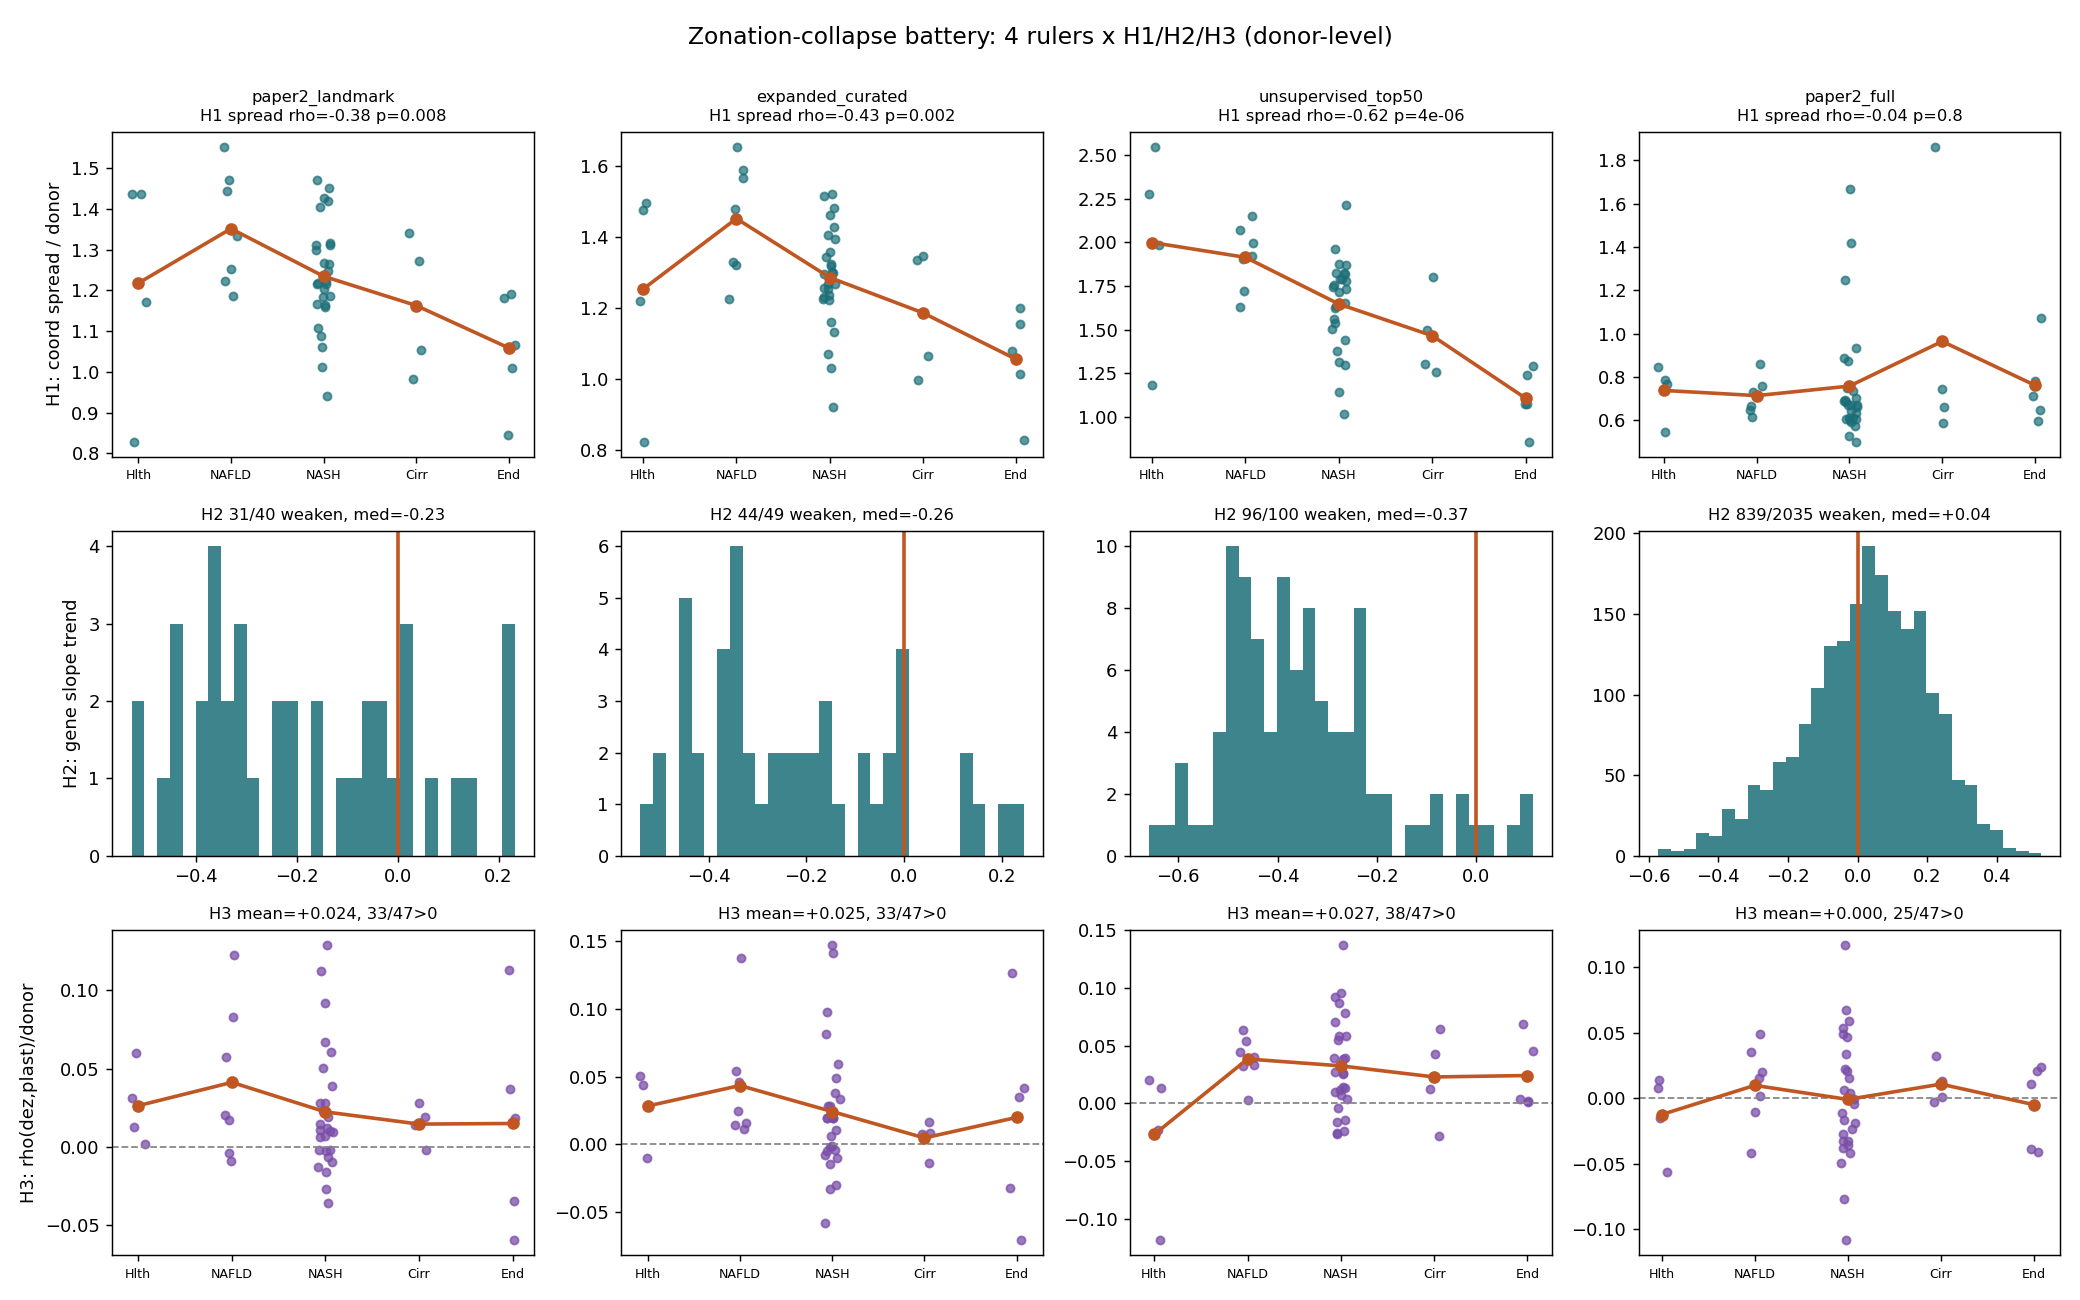
\includegraphics[width=\textwidth]{figures/ruler_panel.png}\end{center}

\section{Discussion}
Three independent constructions --- a published landmark signature, a label-free PCA axis (trained
even on a fully external healthy atlas), and regularized sparse axes --- converge on the same
conclusion: hepatocyte zonation progressively collapses across MASLD, the pericentral Wnt-identity
program leads the loss, and de-zonation is mildly associated with epithelial plasticity. Because
ruler selection was confined to healthy-atlas criteria, the disease findings are genuine transfer
results rather than fitted outcomes.

\section{Limitations}
(i) Donor numbers per stage are imbalanced (4/7/27/4/5), so cirrhosis/end-stage estimates are thin;
all inference is donor-level with bootstrap CIs and permutation nulls to respect this. (ii) Paper~2
per-cell zone labels are an $\eta$-over-landmark reconstruction (Paper~2's own method) --- spatially
grounded but not a physical coordinate; classifier entropy is therefore auxiliary. (iii) The
``full'' unweighted set is a cautionary negative, not a result. (iv) H2b program groupings are
curated and the smaller rulers contain few genes per program, so the gene-rich \texttt{paper2\_full}
table is used for the program comparison.

\section{Conclusions}
Hepatocyte zonation collapses with MASLD stage at the donor level (H1), driven first by the
pericentral Wnt-identity program with nitrogen and xenobiotic metabolism following (H2), and is
weakly coupled to epithelial plasticity (H3). The result is robust to how the ruler is built and to
training the ruler on a fully external healthy atlas.

\vspace{1em}\footnotesize Companion artefacts: per-set dossier \texttt{Zonation\_Ruler\_Report.pdf};
machine tables \texttt{signature\_battery\_summary.csv}, \texttt{selected\_set\_decision.txt},
per-set \texttt{results/tables/<set>/}.
\end{document}
